\section{Esercitazioni} 
\subsection{Esercitazione 21/09/23}
\subsubsection{Costruzione DFA}
Consideriamo l'alfabeto \{a,b\}. 
Realizzare dei DFA che riconoscono i seguenti linguaggi:
\begin{enumerate}
  \item stringhe con un numero dispari di a 
\\ SI ab,aaa,bba,aaba
\\ NO $\epsilon$,aa

\begin{figure}[h]
  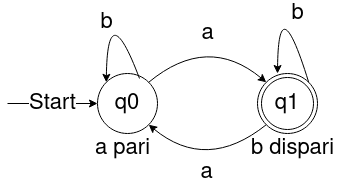
\includegraphics[scale = 0.5]{media/09_21_es1.png}
  \centering
\end{figure}

\item 
stringhe che terminano con bb
\\ SI bb,babb
\\ NO $\epsilon$,ba,a,aba

\begin{figure}[h]
  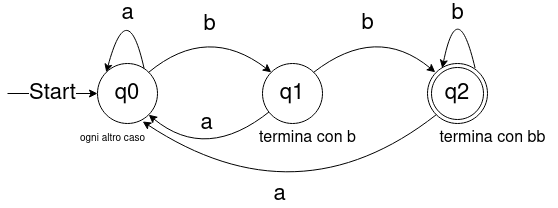
\includegraphics[scale = 0.5]{media/09_21_es2.png}
  \centering
\end{figure}

\newpage
\item stringhe che non terminano con bb
\\ SI $\epsilon$,ba,a,aba
\\ NO bb,babb

\begin{figure}[h]
  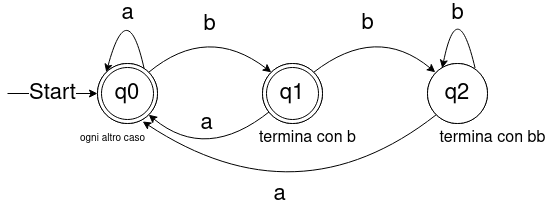
\includegraphics[scale = 0.5]{media/09_21_es3.png}
  \centering
\end{figure}

\newpage
\item stringhe con un numero pari di a ed almeno 3 b
\\ SI bbb,bababb
\\ NO $\epsilon$,bbaa,bababa

\begin{figure}[h]
  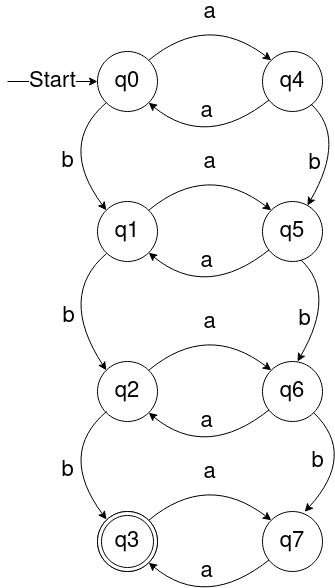
\includegraphics[scale = 0.5]{media/09_21_es4.png}
  \centering
\end{figure}

\newpage
\item stringhe che contengono la sottostringa aaa o la sottostringa aba (contengono almeno una delle due)
\\ SI babab,aaaa,aaaba
\\ NO $\epsilon$,abba,a,b,ab

\begin{figure}[h]
  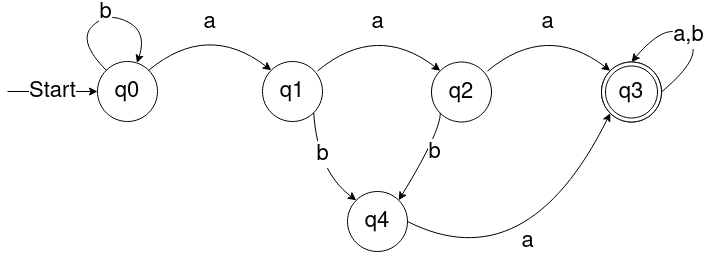
\includegraphics[scale = 0.5]{media/09_21_es5.png}
  \centering
\end{figure}

\item Realizzare un DFA che riconosca il seguente linguaggio su alfabeto \{0,1\}: stringhe che interpretate come numero binario risultano un multiplo di 5 
\\
SI 101,1010,1111,0
\\
NO 111,1,10

\begin{figure}[h]
  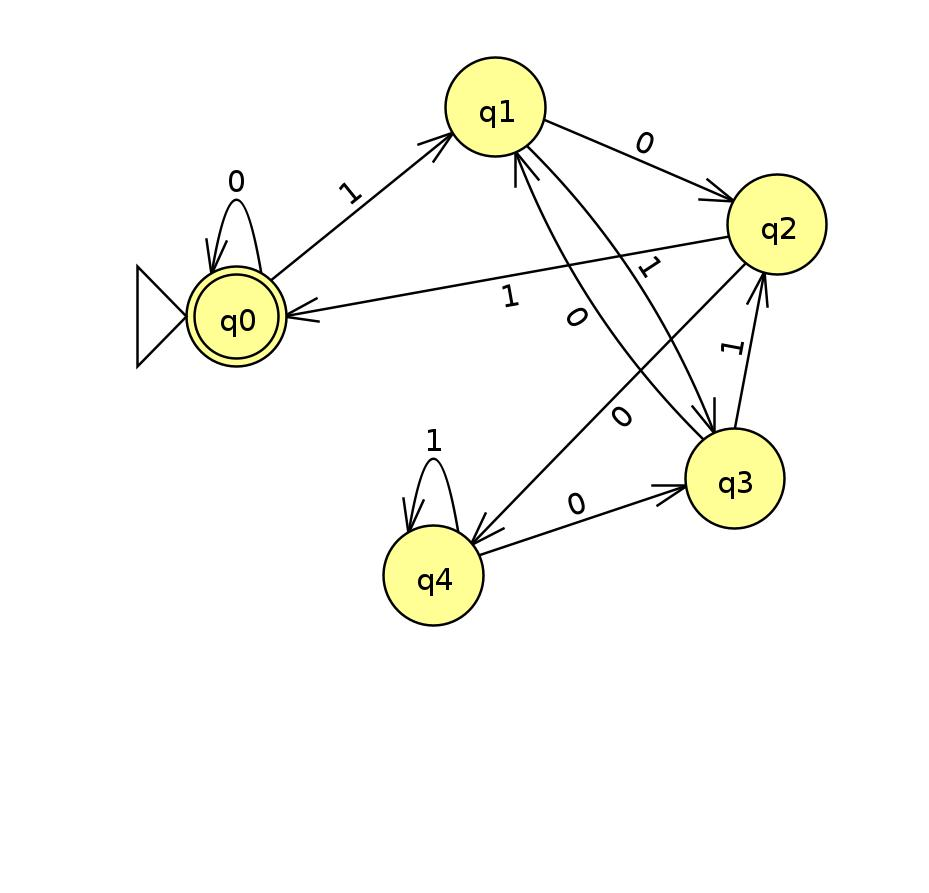
\includegraphics[scale = 0.25]{media/09_21_es6.jpg}
  \centering
\end{figure}
NB: Devi considerare tutti i numeri fino a 5!

\item Sempre considerando alfabeto \{0,1\}, realizzare un DFA che controlla la correttezza delle somme binarie: data la stringa: $a_0 b_0 c_0 a_1 b_1 c_1 ... a_n b_n c_n$ controlla se $a_n...a_1 a_0 + b_n...b_1 b_0 = c_n...c_1 c_0$ (cioè a+b=c con a,b,c numeri binari con stessa lunghezza) 

\begin{figure}[h]
  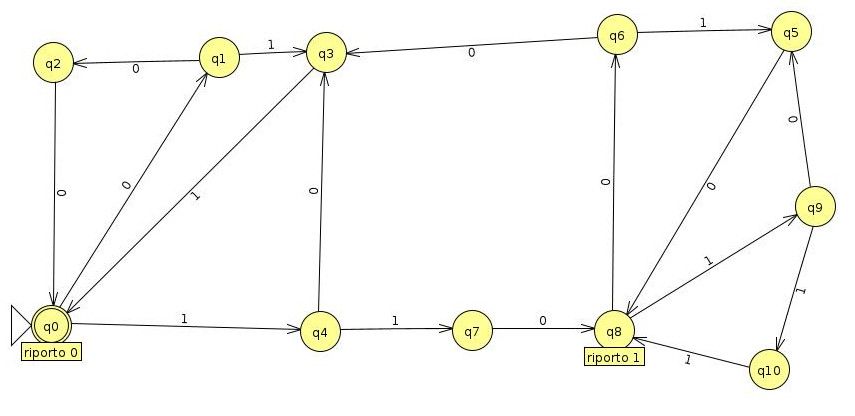
\includegraphics[scale = 0.4]{media/09_21_es7.jpg}
  \centering
\end{figure}

\end{enumerate}

\newpage
\subsubsection{NFA}
\begin{enumerate}
  \item 
    Dato l'alfabeto \{a,b\} realizzare un NFA che riconosce le stringhe che 
    contengono aaa oppure aba
    \\
    SI babab,aaaa,aaaba
    \\
    NO $\epsilon$,abba,a,b,ab

\begin{figure}[h]
  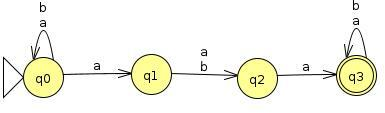
\includegraphics[scale = 0.5]{media/es8.jpg}
  \centering
\end{figure}

  \item Realizzare un NFA che riconosce le stringhe non vuote sull'alfabeto \{0,1,2\} in cui l'ultima cifra appare almeno una volta in precedenza
    \\
    SI 011,121,22,0120
    \\
    NO $\epsilon$,012,20,1

\begin{figure}[h]
  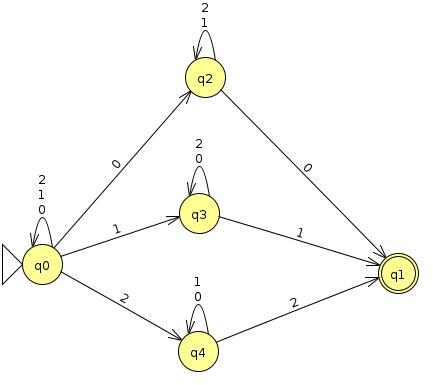
\includegraphics[scale = 0.5]{media/es9.jpg}
  \centering
\end{figure}

\newpage
\item Realizzare un NFA che riconosce le stringhe non vuote sull'alfabeto {0,1,2} in cui l'ultima cifra NON appare in precedenza
\\
SI 012,20,1
\\
NO $\epsilon$,011,121,22,0120

\begin{figure}[h]
  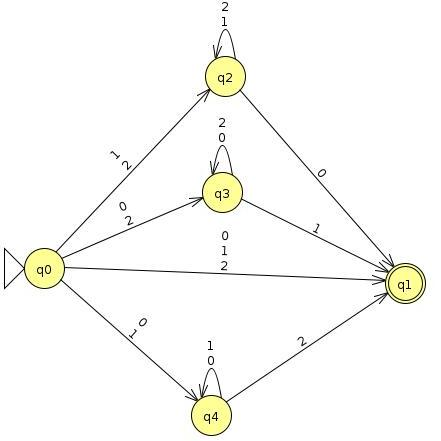
\includegraphics[scale = 0.5]{media/es10.jpg}
  \centering
\end{figure}

\item Dato l'alfabeto {a,b} si consideri l'NFA fatto all'esercizio 1, che riconosce le stringhe che contengono aaa oppure aba. Trasformarlo in DFA.

\begin{figure}[h]
  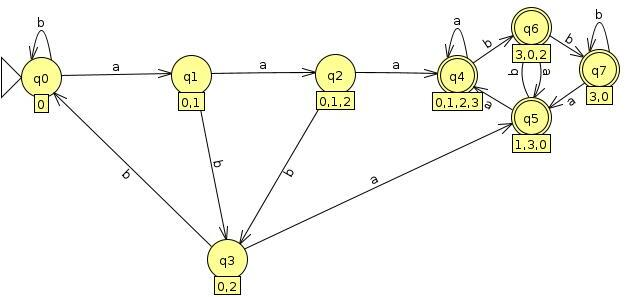
\includegraphics[scale = 0.5]{media/es11.jpg}
  \centering
\end{figure}
\end{enumerate}

\newpage
\subsection{Esercitazione 28/09/23}
\subsubsection{Pumping lemma}
Mostrare che i seguenti linguaggi non sono regolari:
\begin{enumerate}
  \item Linguaggio sull'alfabeto \{a,b\} delle stringhe $a^hb^m$ con $m\geq 2h$
\textbf{Soluzione}
\\ Si supponga per assurdo che L sia regolare.
\\ Deve quindi esistere un DFA A tale che $L=L(A)$.
\\ Quindi, chiamato $n$ il numero degli stati di A, si ha che:

$\exists n>=1: \forall w \in L, |w|\geq n$, $w$ può essere scomposta in $w=xyz$ con $|y|>0, |xy| \leq n$, 
$xy^kz$ appartiene ad L per ogni $k \geq 0$
\\ (PUMPING LEMMA)
\vspace{5mm}
\\ Considero la stringa $w=a^n b^{2n}$, e decido che la stringa $y$ è composta da sole $a$ e almeno una. Prendiamo $k>2$ allora la stringa risultate è $z=xyyz$, li numero delle $a$ è aumentato ma il numero delle $b$ no, paradosso.
Si può concludere che $w \notin L$ quindi L non è regolare.

\item Linguaggio delle parentesi tonde bilanciate; cioè, delle stringhe, sull'alfabeto composto dai due simboli "(" e ")", che sono espressioni Exp fatte come segue.
\\ Una Exp e' nella forma: ( Exp1 ) oppure Exp1 Exp2 oppure $\epsilon$
\\ Esempi di stringhe del linguaggio: 
\\ ()()((()))
\\ (()())
\\ (())((()))
\\ Esempi di stringhe non del linguaggio: 
\\ )(
\\ (()

\vspace{5mm}
Formalmente dimostro che $L=\{ "(",")"\}$ non è regolare:
\\ Si supponga per assurdo che L sia regolare.
\\ Deve quindi esistere un DFA A tale che $L=L(A)$.
\\ Quindi, chiamato $n$ il numero degli stati di A, si ha che:

$\exists n>=1: \forall w \in L, |w|\geq n$, $w$ può essere scomposta in $w=xyz$ con $|y|>0, |xy| \leq n$, 
$xy^kz$ appartiene ad L per ogni $k \geq 0$
\\ (PUMPING LEMMA)
\vspace{5mm}

Prendiamo la stringa $w=(^n)^n$, e decido che $y$ è composta da "(" e che $k>2$. Allora la stringa $z=xyyz$ ma così ho più "(" che ")", assurdo.

Si può concludere che $w \notin L$ quindi L non è regolare.


\item Linguaggio sull'alfabeto binario delle stringhe del tipo $xy$ dove $y$ coincide con il complemento di $x$ (0 diventano 1, 1 diventano 0). 
  \\ Sinceramente il testo mi confonde e alla fine dei conti è uguale alle 2 dimostrazioni precedenti, quindi non la metto.

\item Linguaggio sull'alfabeto binario delle stringhe del tipo ww

\vspace{5mm}
Formalmente dimostro che $L=\{ w^2n \}$ non è regolare:
\\ Si supponga per assurdo che L sia regolare.
\\ Deve quindi esistere un DFA A tale che $L=L(A)$.
\\ Quindi, chiamato $n$ il numero degli stati di A, si ha che:

$\exists n>=1: \forall w \in L, |w|\geq n$, $w$ può essere scomposta in $w=xyz$ con $|y|>0, |xy| \leq n$, 
$xy^kz$ appartiene ad L per ogni $k \geq 0$
\\ (PUMPING LEMMA)
\vspace{5mm}

Prendiamo la stringa $s=w^2n$, e decido che $y$ è composta da $w$ e che $k>0$. Allora la stringa $z=xyz$ ma così ho più $w$ dispari.

Si può concludere che $s \notin L$ quindi L non è regolare.
\end{enumerate}

\subsubsection{Espressioni regolari}
\begin{enumerate}
\item Considerare l'espressione regolare 0*(0+11)1*. Dire quale linguaggio rappresenta.

  \[ L=\{ 0^n \times 1^m | n \geq 0, m \geq 0, x \in \{0,11\} \} \]
  
\newpage
\item Considerare l'espressione regolare 1*0+0*1. Trasformalo in un $\epsilon$-NFA.
  \begin{figure}[ht]
    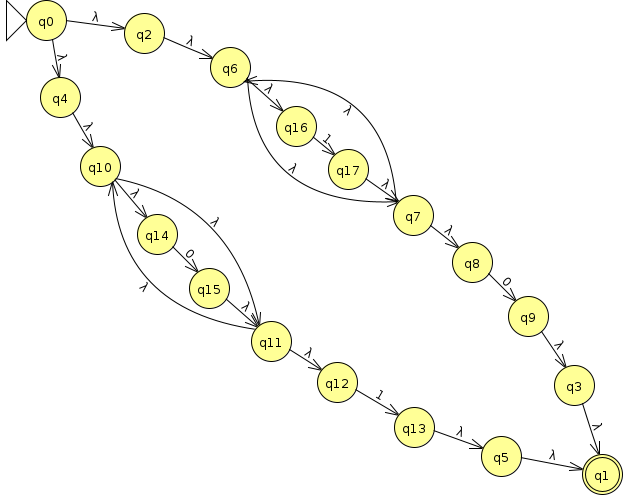
\includegraphics[scale =0.4]{media/esercizio3jflap.jff.png}
    \centering
  \end{figure}

\item Trasformare in RE il seguente automa

  \begin{figure}[ht]
    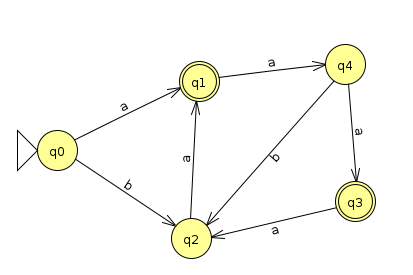
\includegraphics[scale =0.4]{media/nfa2re.jff.png}
    \centering
  \end{figure}
  (a+ba)(aba+aaaa)*+(a+ba)(aba)*aa(aa(aba)*aa)*

  È una banale applicazione della formula


\item 5 Si consideri l'alfabeto \{a,b\}.

  Definisci un RE che accetta un numero pari di $a$ seguito da un numero di $b$ che diviso per 3 da' resto 2

  (aa)*+bb(bbb)*
\end{enumerate}
\subsection{Esercitazione 05/10/23}
\subsubsection{CFG}
\begin{enumerate}
  \item Definire una grammatica libera dal contesto (CFG) per i seguenti linguaggi sull'alfabeto \{a,b,c\}:
    \begin{enumerate}
      \item linguaggio delle stringhe $a^n \; b^{2n}$ (mostrare che "aabbbb" è derivabile dalla CFG)

        $S \rightarrow aSbb$

        $S \rightarrow \lambda$
      \item linguaggio delle stringhe $(abc)^n \; (cba)^n$

        $S \rightarrow abc S cba$

        $S \rightarrow \lambda$
      \item linguaggio delle stringhe $a^n b^m$ in cui $n \leq m$

        $S \rightarrow a S b$

        $S \rightarrow S b$

        $S \rightarrow \lambda$
      \item linguaggio delle stringhe $a^n b^m c^n$ con n pari e m dispari

        $S \rightarrow aaScc$

        $S \rightarrow bA$

        $A \rightarrow bbA$

        $S \rightarrow \lambda$
      \item linguaggio delle stringhe $a^n b^m c^p$ in cui $n \leq m+p$

        $S \rightarrow aSc$
        
        $S \rightarrow Sc$

        $B \rightarrow \lambda$

        $S \rightarrow B$

        $B \rightarrow aBb$

        $B \rightarrow Bb$
    \end{enumerate}

  \item  Dire se la CFG del punto "e" dell'esercizio 3 è ambigua o meno. In caso affermativo mostrare una stringa generata dalla CFG che abbia (almeno) due alberi sitattici/derivazioni canoniche sinistre. Mostrare tali alberi sintattici e le corrispondenti derivazioni canoniche sinistre. 

    È ambigua, ho due derivazioni di $abc$

    $S \rightarrow aSc$ \hspace{3cm} $S \rightarrow Sc$

    $S \rightarrow aBc$ \hspace{3cm} $S \rightarrow aBbc$

    $S \rightarrow abc$ \hspace{3cm} $S \rightarrow abc$

  \item Esercizio su minimizzazione DFA. Effettuare (a mano con l'algoritmo riempi-tabella visto a lezione) la minimizzazione dell'automa in exMinimization.jff

\end{enumerate}
